% =======================================================================================
\section{Architecture and Training}
\label{sec:architecture}
% =======================================================================================
% 2026-11-22 (user): split from the former Method section, with more on the MMDiT and its place
% in the diffusion literature, and a subsection on the embeddings.

The flow of \cref{sec:flow} asks one network for two outputs: the frame of a window from its data
alone, and the endpoint of every source given a point on the path. The first is a regression on a
sequence, and the second is the task of a diffusion model, to denoise a few tokens under a
condition that is itself a long sequence. We take the network from that literature and change it
where a posterior differs from an image.

\subsection{A One-Way Multimodal Diffusion Transformer}
\label{sec:method-network}\label{sec:gw-tokens}

\paragraph{Diffusion transformers.}
The network of a diffusion or flow model
\citep{sohl2015deep,ho2020denoising,song2021score,lipman2023flow} takes a noised sample, its
position on the path and a condition. The diffusion transformer of \citet{peebles2023scalable} cuts
the sample into patch tokens and runs a transformer over them. The time and the class label are not
tokens: they shift and scale every layer normalisation, and gate residual branches that start as
the identity. The \ac{mmdit} of \citet{esser2024scaling}, built for text-to-image rectified flows
\citep{liu2023flow}, extends this to a condition that is a sequence. The text tokens and the
image tokens keep their own weights, as two streams, and meet in one attention over both
sequences, so each modality reads the other in every block.

Our problem has the same shape. The sample is the set of sources, $S$ tokens of eight coordinates
each, and the condition is the data, a longer sequence of tokens (\cref{sec:method-embeddings}).
The \ac{mmdit} fits it in three respects. Separate weights let the data stream, which holds
whitened spectra, and the source stream, which holds coordinates, be built differently. Joint
attention lets every source read the data and the other sources in one operation, which is what
a joint posterior of overlapping sources needs. And the conditioning by modulation carries the flow
time and the window to every layer without spending a token on them.

\paragraph{Four streams.}
\Cref{fig:network-architecture} shows the network. Each stream has its own normalisations,
attention projections and feed-forward maps. The \emph{data} stream holds the tokens of the
window. A \emph{register} stream runs beside it, one token per source slot in the sense of
\citet{darcet2024vision}, and a head reads the slot's frame $(\mu,\log\sigma)$ from its register
(\cref{app:network-frame}). The \emph{source} stream holds one token per slot, and a head reads
the endpoint $\hat Z_1$ and $\log\tau$ from it (\cref{app:network-head}). A \emph{sink} stream of
\NetworkSinksWord{} tokens runs beside the sources and gives their attention somewhere to go other
than the data \citep{xiao2024efficient,darcet2024vision}. The conditioning vectors modulate every
normalisation and gate every residual branch, as in \citet{peebles2023scalable}: $\nu_f$, from the
window alone, in the data and register streams, and $\nu$, from the flow time and the window, in
the source and sink streams.

\begin{figure*}[t]
  \centering
  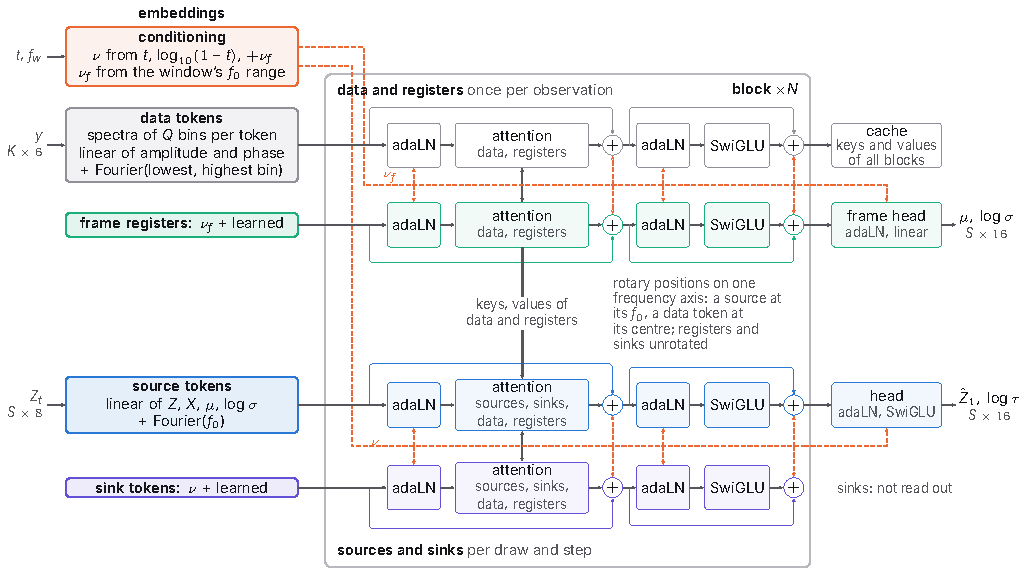
\includegraphics[width=\textwidth]{figures/architecture.pdf}
  \caption{The network: four streams, each with its own normalisations, attention projections and
  feed-forward. The source stream (blue) has one token per source slot, in order of $f_0$, and the
  sink stream (violet) \NetworkSinksWord{} tokens; they attend jointly. The data stream (grey) has
  one token per \NetworkPatch{} frequency bins of the window, and the register stream (green) one
  frame register per slot, which the frame head reads; they attend jointly. Conditioning (orange, dashed) modulates every normalisation and residual gate:
  $\nu$ from the flow time and the window in the source stream and head, $\nu_f$ from the window
  alone in the data stream, the registers and the frame head. The data side never reads the
  sources, so its keys and values and the frame are computed once per observation and serve every
  draw and sampler step. Rotary positions place each source at its $f_0$ and each data token at its
  centre frequency.}
  \label{fig:network-architecture}
\end{figure*}

\paragraph{One-way attention.}
A window is a long sequence but holds few sources, and a posterior needs many draws, each followed
over many sampler steps. In the \ac{mmdit} the text stream reads the image tokens and the time, so
the whole network runs again at every step. Ours reads in one direction. With queries $q$, keys
$k$ and values $v$ of the data ($y$), register ($r$), source ($x$) and sink ($s$) streams, each
block computes
\begin{equation}
\begin{aligned}
  [o^y; o^r] &= \mathrm{Attn}\bigl([q^y; q^r]; [k^y; k^r], [v^y; v^r]\bigr),\\
  [o^x; o^s] &= \mathrm{Attn}\bigl([q^x; q^s]; [k^x; k^s; k^y; k^r], [v^x; v^s; v^y; v^r]\bigr),
\end{aligned}
  \label{eq:network-oneway}
\end{equation}
so the data and the registers attend to each other only, and the sources and the sinks attend to
everything (\cref{eq:network-block}). The data side is conditioned on the window alone, never on
the flow time or the sources. Its keys and values in every block and the frame therefore depend on
$(y,\fw)$ only: they are computed once per window and serve every draw and every sampler step. In
size B, encoding a full-band window costs \NetworkEncodeOverDecodeFull{} times one evaluation of
the source side on the cache (\cref{app:network-blocks}), and a draw takes
\NetworkSampleEvals{} such evaluations. \Cref{tab:network-sizes} gives the sizes; all results use
size B, with \NetworkBBlocks{} blocks of width \NetworkBWidth{} and \num{\NetworkBTotalFull}
parameters.

\subsection{Embeddings}
\label{sec:method-embeddings}

An image enters a diffusion transformer as patches of pixels with a position each. Our two
sequences are a spectrum and a set of coordinates, and what each token holds decides what the
attention can resolve: a posterior a small fraction of a bin wide requires frequency at sub-bin
resolution in every embedding. \Cref{tab:network-embeddings} lists what each token is built from,
and \cref{app:network} gives the details.

\paragraph{Data tokens.}
The window is cut into patches of \NetworkPatch{} consecutive frequency bins, one token each:
\NetworkTokensNarrow{} tokens in the narrow band and \NetworkTokensFull{} in the full band. An
inverse Fourier transform over the patch turns its bins into as many time samples per channel, an
\ac{stft} with the tokens as its bands (\cref{eq:network-stft}). The transform is critically
sampled and untapered, so it is invertible and keeps the noise white. In it a source's sub-bin
frequency is a phase slope over the samples, its initial phase the intercept, and the annual
modulation that carries its sky position a slow evolution in time. Whitened samples of loud
sources are far above the unit noise, so each complex sample enters as a compressed amplitude,
$\operatorname{asinh}\lvert\check y\rvert$, and a gated phase,
$\check y/\sqrt{1+\lvert\check y\rvert^2}$, mapped linearly to the token
(\cref{app:network-input}).

\paragraph{Source tokens.}
A source token is a linear map of the slot's current point in the frame, $Z_s$, the same point in
the flow coordinates, $X=\mu+\sigma Z_s$, the higher harmonics of its two helicity phases, and its
frame $(\mu,\log\sigma)$, which it reads through a stop-gradient (\cref{app:network-sources}). The
token carries no label of its slot and every map is shared across sources, as in set transformers
\citep{zaheer2017deep,lee2019set}; a source is told apart by its frame and its frequency.

\paragraph{Frequency.}
Whitening and windowing remove the absolute frequency, on which the width of a source's response
and the prior's drift depend. It enters three times as sinusoids with octave-spaced periods, from
\NetworkFreqFinest{} of a bin up to past twice the top of the band: the edges of each data token,
the $f_0$ of each source token, and the edges of the window in $\nu_f$. Inside the attention,
rotary embeddings \citep{su2024roformer,miyato2024gta} turn the queries, keys and values of the
data and source tokens by their frequency, a data token's centre and a source's $f_0$. A score
then depends on how far apart two tokens are in frequency, so a source finds the data near its own
$f_0$ wherever the window lies in the band (\cref{app:network-positions}). The registers and the
sinks are learned vectors without a position.

\paragraph{Flow time.}
The time enters $\nu$ as sinusoids of $s$ and of $\log_{10}(1-s)$, the latter clipped at
\NetworkTimeDecades{} decades. The second input resolves the end of the path, where the fine
structure of a narrow posterior forms (\cref{app:network-conditioning}).

\subsection{Training}
\label{sec:method-training}\label{sec:gw-training}

Every training window is simulated afresh, on the device and inside the compiled training step, so
no window is seen twice (\cref{app:priors-training}). A window starts from a centre $\fw$. Centres
drawn from the catalogue's $f_0$ marginal would mostly hold no visible source, so we weight the
marginal by the chance that a source there is visible (\cref{eq:priors-window}) and draw
\qty{\PriorsUniformWindowsPercent}{\percent} of the centres log-uniformly over the band, so that
training also sees windows with nothing to resolve. The weights choose which windows training sees,
not what their sources are, so the posterior given a window is unchanged (\cref{app:priors-window}).
The window then receives $S$ sources drawn from $\pi_w$ (\cref{eq:priors-window-prior}), their
$R$-bin responses and a noise draw (\cref{eq:noise-data}), and is whitened; the sources enter the
flow coordinates in order of $f_0$. Unlike \citet{delmond2026neural}, who precompute a bank of
responses and keep sources with an \ac{snr} between 10 and 100, we apply no cut: most of a window's
sources lie below the noise, and for them the flow must return the prior. The simulation takes
\qty{\PriorsNarrowDrawShare}{\percent} of a training step in the narrow band and
\qty{\PriorsFullDrawShare}{\percent} in the full band (\cref{tab:priors-bands}).

A batch holds \TrainingObservations{} windows, each with \TrainingDraws{} draws of time and base
point that share its cached data side (\cref{app:training-batch}). The optimiser is Muon
\citep{jordan2024muon,liu2025muon} for the hidden weight matrices and AdamW for the rest, with a
linear warmup, a constant learning rate and a cooldown to zero \citep{hagele2024scaling}
(\cref{app:training}). Each run trains on one A100 \ac{gpu}, for \ResultsNarrowHours\,h on the
narrow band and \ResultsFullHours\,h on the full band (\cref{tab:results-runs}), and is evaluated at
the checkpoint with the lowest loss on held-out windows (\cref{app:evaluation-weights}).
